\chapter{Meta}

\section{Hintergrund}

Wir leben in einer Gesellschaft, in der jährlich ca. 1.3 Milliarden Tonnen an Lebensmitteln, die für den Verzehr geeignet sind, aufgrund ihrer Abweichung von Marktnormen, Überproduktion oder aufgrund von falscher Interpretation des Begriffes \glqq Mindesthaltbarkeitsdatum\grqq\space weggeworfen werden.

Besonders Restaurants und Hotels mit einem All-You-Can-Eat-Buffet tragen einen signifikanten Teil zu dieser enormen Verschwendung essbarer Nahrungsmittel bei.

Genau hier kommt \textbf{Sokka} ins Spiel und soll für dringend nötige Veränderung sorgen. Durch die Möglichkeit, Bestellungen von Kunden einfach verwalten zu können, haben Köche, die auf die Dienste von Sokka zurückgreifen einen besseren Überblick darüber, welche Menge an bestimmten Gerichten zubereitet werden müssen.\\
Auf diese Weise kann nachhaltig verhindert werden, dass zu viel gekocht und letztendlich dann doch entsorgt wird.

\section{Namensherkunft}

Der Name \textbf{Sokka} stammt ursprünglich aus der Serie \textit{Avatar: Der Herr der Elemente}. In jener Serie ist Sokka ein Nebencharakter, der ständig über sein konstantes Bedürfnis zu essen spricht und eine Vorliebe dafür hat, exotische Spezialitäten in besonders großen Mengen zu probieren.

Da sich dieses Projekt ebenso um die verschiedenen Speisen und Gerichte eines Restaurants und deren Verwaltung dreht, wurde das System nach dieser Figur zu benannt.

\begin{figure}[H]
    \begin{center}
        
\includegraphics[width=0.22\textwidth]{images/Intro/Sokka.png}
        \caption{Der Charakter \textbf{Sokka} aus der Serie \textit{Avatar: Der Herr der Elemente}}
        \cite{nickelodeon2005}
    \end{center}
\end{figure}

\newpage

\section{Projektlogo}

Das Markenzeichen des vorher genannten Charakters \textbf{Sokka} ist der Boomerang in seiner Hand. Dieser Boomerang wurde dann in Form eines grinsenden Gesichts zum Logo des Projekts.

\begin{figure}[H]
    \centering
    \hfill
    \subfigure[Sokkas Boomerang~\cite{aguilar2020}]{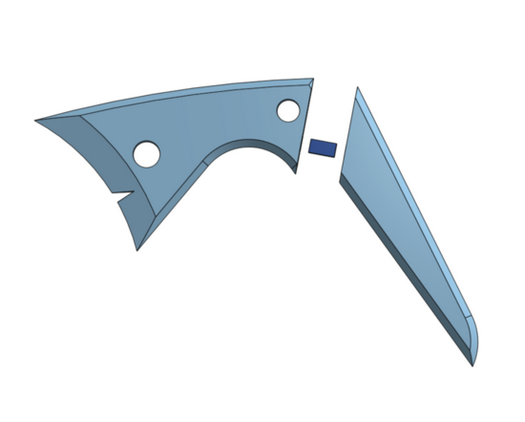
\includegraphics[width=0.4\textwidth]{images/Intro/Boomerang.png}}
    \hfill
    \subfigure[Sokka Projektlogo]{
\includegraphics[width=0.4\textwidth]{images/sokka.png}}
    \hfill
    \caption{Sokkas Boomerang und das Projektlogo}
\end{figure}